\documentclass[reprint,english,notitlepage]{revtex4-1}  % defines the basic parameters of the document

% if you want a single-column, remove reprint

% allows special characters (including æøå)
\usepackage[utf8]{inputenc}
\usepackage[english]{babel}

\usepackage{siunitx}

%% note that you may need to download some of these packages manually, it depends on your setup.
%% I recommend downloading TeXMaker, because it includes a large library of the most common packages.

\usepackage{physics,amssymb}  % mathematical symbols (physics imports amsmath)
\usepackage{graphicx}         % include graphics such as plots
\usepackage{xcolor}           % set colors
\usepackage{hyperref}         % automagic cross-referencing (this is GODLIKE)
\usepackage{tikz}             % draw figures manually
\usepackage{listings}         % display code
\usepackage{subfigure}        % imports a lot of cool and useful figure commands

\newcommand{\vect}[1]{\boldsymbol{#1}}

% defines the color of hyperref objects
% Blending two colors:  blue!80!black  =  80% blue and 20% black
\hypersetup{ % this is just my personal choice, feel free to change things
    colorlinks,
    linkcolor={red!50!black},
    citecolor={blue!50!black},
    urlcolor={blue!80!black}}

%% Defines the style of the programming listing
%% This is actually my personal template, go ahead and change stuff if you want
\lstset{ %
	inputpath=,
	backgroundcolor=\color{white!88!black},
	basicstyle={\ttfamily\scriptsize},
	commentstyle=\color{magenta},
	language=Python,
	morekeywords={True,False},
	tabsize=4,
	stringstyle=\color{green!55!black},
	frame=single,
	keywordstyle=\color{blue},
	showstringspaces=false,
	columns=fullflexible,
	keepspaces=true}


%% USEFUL LINKS:
%%
%%   UiO LaTeX guides:        https://www.mn.uio.no/ifi/tjenester/it/hjelp/latex/ 
%%   mathematics:             https://en.wikibooks.org/wiki/LaTeX/Mathematics

%%   PHYSICS !                https://mirror.hmc.edu/ctan/macros/latex/contrib/physics/physics.pdf

%%   the basics of Tikz:       https://en.wikibooks.org/wiki/LaTeX/PGF/TikZ
%%   all the colors!:          https://en.wikibooks.org/wiki/LaTeX/Colors
%%   how to draw tables:       https://en.wikibooks.org/wiki/LaTeX/Tables
%%   code listing styles:      https://en.wikibooks.org/wiki/LaTeX/Source_Code_Listings
%%   \includegraphics          https://en.wikibooks.org/wiki/LaTeX/Importing_Graphics
%%   learn more about figures  https://en.wikibooks.org/wiki/LaTeX/Floats,_Figures_and_Captions
%%   automagic bibliography:   https://en.wikibooks.org/wiki/LaTeX/Bibliography_Management  (this one is kinda difficult the first time)
%%   REVTeX Guide:             http://www.physics.csbsju.edu/370/papers/Journal_Style_Manuals/auguide4-1.pdf
%%
%%   (this document is of class "revtex4-1", the REVTeX Guide explains how the class works)


%% CREATING THE .pdf FILE USING LINUX IN THE TERMINAL
%% 
%% [terminal]$ pdflatex template.tex
%%
%% Run the command twice, always.
%% If you want to use \footnote, you need to run these commands (IN THIS SPECIFIC ORDER)
%% 
%% [terminal]$ pdflatex template.tex
%% [terminal]$ bibtex template
%% [terminal]$ pdflatex template.tex
%% [terminal]$ pdflatex template.tex
%%
%% Don't ask me why, I don't know.

\begin{document}
\title{Regression Analysis of a Bivariate Function}   % self-explanatory
\author{Aron Jansson Nordberg}               % self-explanatory
\date{\today}                             % self-explanatory
\noaffiliation                            % ignore this
\begin{abstract}                          % marks the beginning of the abstract
We have studied the application of the three machine learning methods Ordinary Least Squares, Ridge and LASSO on the Franke function. We have approximated them using polynomials, and tuned the hyperparameters to find the best fit. We have also employed resampling techniques when determining the hyperparameters. Ordinary Least Squares yielded the best results, with polynomials of degree 5.% the body of the abstract
\end{abstract}                            % marks the end of the abstract
\maketitle                                % creates the title, author, date & abstract


% the fundamental components of scientific reports:
\section{Introduction}
All the code and material for this report is to be found in the github repository:
\texttt{https://github.com/aronjn/FYS-STK3155}

In machine learning, a major topic of interest is supervised learning. We are given a data set which consists of inputs/predictors $X$ and outputs/responses $Y$. The goal of supervised learning is to determine a function/model that maps the input to the output, that is finding an $f$ such that $Y = f(X)$. When the output is a continuous function, the we call it a regression problem.

In this project, we shall be concerned with fitting models to bivariate functions, $z = f(x, y)$, also called terrain functions. We will consider the Franke function, and test three regression methods: Ordinary Least Squares, Ridge, and LASSO. We will also employ the resampling methods train-test split and $K$-fold cross validation. We will test the results of each method by computing the Mean Squared Errors and the $R^2$ scores.

The model that we will study, and use to approximate the bivariate functions, are linear combinations of polynomials in $x$ and $y$.

\section{Theory}

\subsection{Regression Methods}

\subsubsection{Ordinary Least Squares}
Consider a data set, where the $N$ responses are collected in the $N$ vector $\vect{z}$. We will assume that each entry can be expressed as a linear combination of polynomials in $x$ and $y$. Let $\hat{\vect{z}}$ be our approximation, and let $\vect{\beta}$ be a $p$ vector, which contains the weights to each of the $p$ polynomials for each of the $N$ entries. The design matrix $X$ is an $N \times p$ matrix, where each row corresponds to an entry in $\vect{z}$ and contains each of the $p$ polynomials as columns. We can now write out approximation as the matrix equation:
\begin{equation} \label{model}
	\hat{\vect{z}} = X\vect{\beta}
\end{equation}
We will determine quality of our approximation by computing the Mean Squared Error ($MSE$), given by
\begin{equation} \label{MSE_cost}
	MSE = \frac{1}{N}\left(\vect{z} - \hat{\vect{z}} \right)^T \left(\vect{z} - \hat{\vect{z}} \right)
\end{equation}
This is our cost function. We want to minimize \ref{MSE_cost}, so we take its derivative with respect to the weights $\vect{\beta}$, using \ref{model}.

\begin{align*}
	MSE &= \frac{1}{N}\left(\vect{z} - X\vect{\beta} \right)^T \left(\vect{z} - X\vect{\beta} \right)\\
	\frac{\partial}{\partial \vect{\beta}} MSE 	&= \frac{1}{N}\left(\vect{0} - X \right)^T \left(\vect{z} - X\vect{\beta} \right) + \left(\vect{z} - X\vect{\beta} \right)^T \left(\vect{0} - X \right)\\
	&= \frac{1}{N} \left[-X^T \left(\vect{z} - X\vect{\beta} \right) - \left(\vect{z} - X\vect{\beta} \right)^T X \right]\\
	&= \frac{1}{N} \left[-X^T \left(\vect{z} - X\vect{\beta} \right) - X^T\left(\vect{z} - X\vect{\beta} \right) \right]\\
	&= \frac{1}{N} \left[-2X^T \left(\vect{z} - X\vect{\beta} \right) \right]
\end{align*}
We now set this equal to $\vect{0}$ and solve for $\vect{\beta}$.
\begin{align*}
	\frac{\partial}{\partial \vect{\beta}} MSE 	&= \vect{0}\\
	\frac{1}{N} \left[-2X^T \left(\vect{z} - X\vect{\beta} \right) \right] &= \vect{0}\\
	X^T \left(\vect{z} - X\vect{\beta} \right) &= \vect{0}\\
	X^TX\vect{\beta} &= X^T\vect{z}
\end{align*}
Assuming that $X^TX$ is non-singular, meaning it is invertible, we have an explicit solution for the values of $\vect{\beta}$ that minimizes \ref{MSE_cost}.
\begin{equation} \label{ols}
	\vect{\beta} = \left( X^TX \right)^{-1}X^T\vect{z}
\end{equation}

\subsubsection{Ridge}
In cases where $X^TX$ is near-singular, to where it might cause computational problems, we can add a penalty term to its diagonal. This will increase the bias of our model.

Our cost function now looks like this
\begin{equation} \label{ridge_cost}
	C = \frac{1}{N}\left(\vect{z} - \hat{\vect{z}} \right)^T \left(\vect{z} - \hat{\vect{z}} \right) + \lambda \vect{\beta}^T\vect{\beta}
\end{equation}
where $\lambda$ is a so-called hyperparameter. Just like with OLS, our goal now is to minimize \ref{ridge_cost} by taking its derivative, setting it equal to $\vect{0}$ and solving for $\vect{\beta}$. Here we state the result
\begin{equation} \label{ridge_beta}
	\vect{\beta} = \left( X^TX + \lambda I_p \right)^{-1}X^T\vect{z}
\end{equation}
where $I_p$ is the $p \times p$ identity matrix. We see that it is quite similar to \ref{ols}, but we now have an additional parameter $\lambda$ that must be determined. This is usually done with a grid search, where a range of values for $\lambda$ are used to generate models, which are tested using $MSE$ and/or $R^2$. The adding of terms to the model is called regularization.

\subsubsection{LASSO}
The method Least Absolute Shrinkage and Selection Operator (LASSO) is similar to Ridge, but the cost function is now
\begin{equation} \label{cost_lasso}
	C = \frac{1}{N}\left(\vect{z} - \hat{\vect{z}} \right)^T \left(\vect{z} - \hat{\vect{z}} \right) + \lambda \sqrt{\vect{\beta}^T\vect{\beta}}
\end{equation}
This time, our previous strategy will no longer work, and we cannot achieve an analytical expression for $\vect{\beta}$. Instead we must perform the computations in a grid search, and determine the $\vect{\beta}$ that minimizes \ref{cost_lasso}.

\subsection{Resampling Methods}
In order to avoid overfitting, that is that our model is fit only to predict the outcomes of the training data used to make it, and not general enough to be applied to new data sets, where the outcome may not be known in advance, we must perform resampling techniques for quality checks.
\subsubsection{Train-Test Split}
In this method, the training data is split into data used for training the model ($X_{train}$ and $\vect{z}_{train}$), and data used for testing ($X_{test}$ and $\vect{z}_{test}$). The given regression method then uses the training data to estimate a $\vect{\beta}$, which is then used to estimate out approximation
\begin{align*}
	\hat{\vect{z}} = X_{test}\vect{\beta}
\end{align*}
Which is then evaluated against $\vect{z}_{test}$ using, for example, $MSE$.

\subsubsection{$K$-Fold Cross Validation}
This method is quite similar to train-test split, but instead of splitting the data set just once, we iterate through all possible divisions (called folds). For example, given $K = 10$, we would split the data set into 10 equal folds, use 9 of them to train our model and test on the remaining 1. The results would be evaluated with $MSE$. Then another one is used as test data while the rest is trained, and so it continues until all combinations have been done. The average $MSE$ is then computes, and is a measure for how good the model did, and it makes sure it is not prone to overfitting.

Figure \ref{kfold} illustrates the process.

\begin{figure}[h]
    \centering
    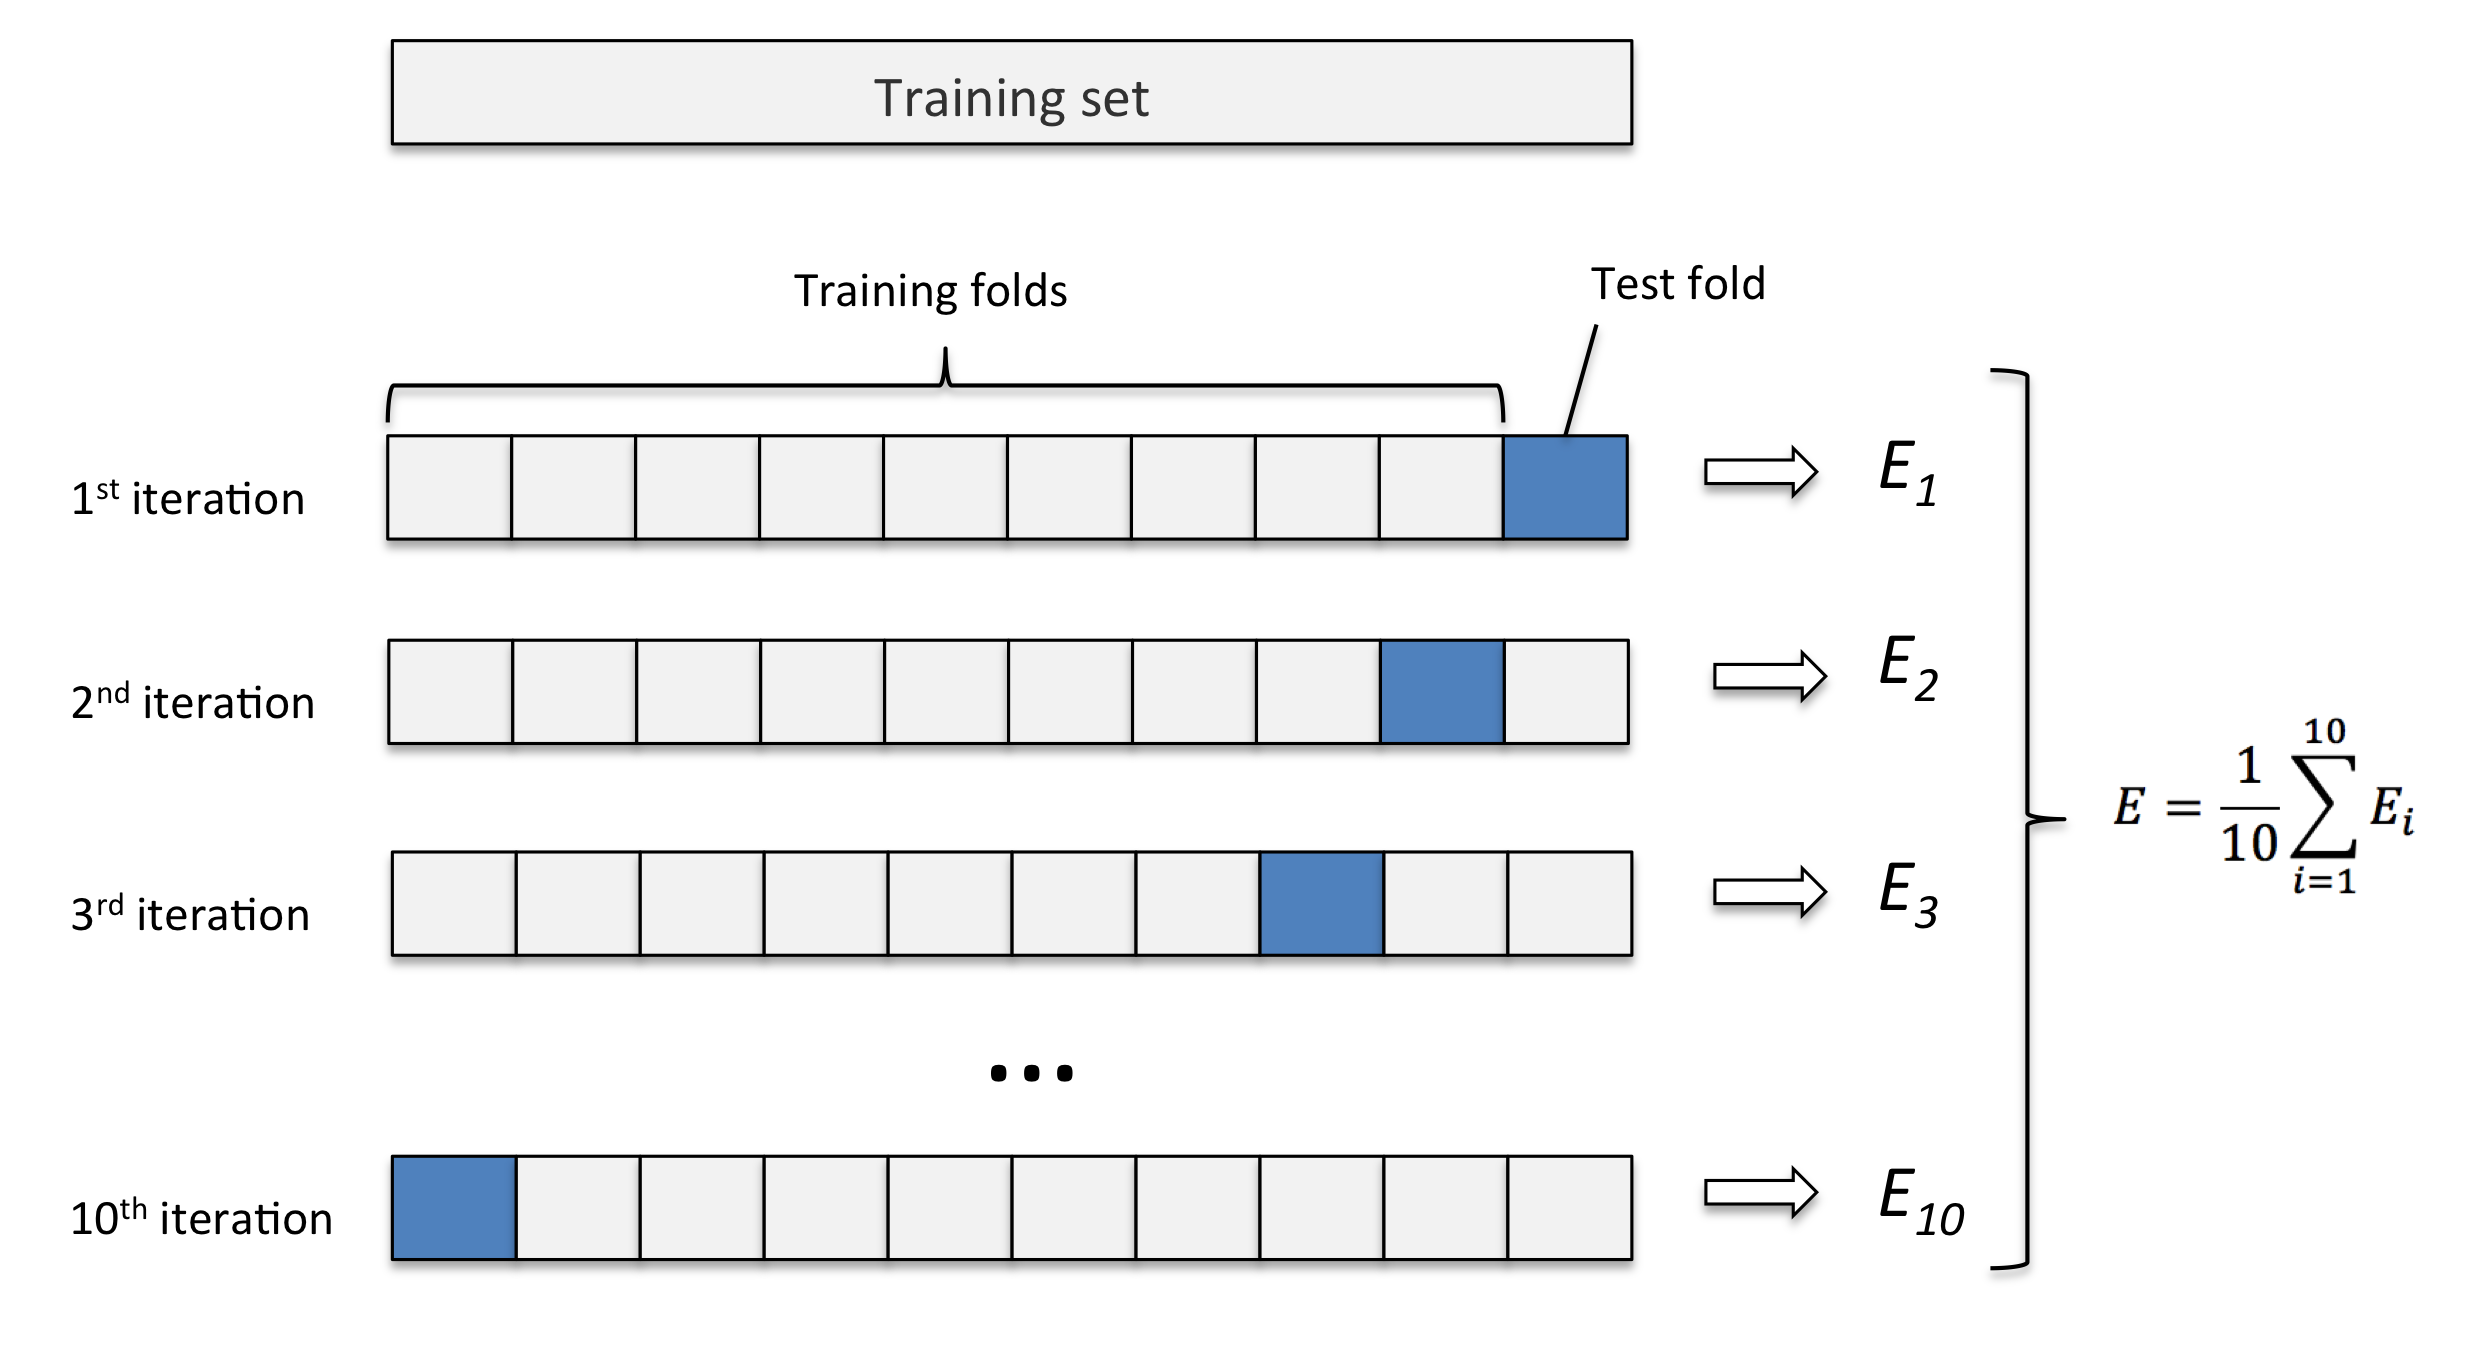
\includegraphics[width=0.50\textwidth]{kfold.png}
    \caption{Illustration of $K$-fold cross validation. Source: https://miro.medium.com/max/6542/1*me-aJdjnt3ivwAurYkB7PA.png}
    \label{kfold}
\end{figure}


\subsection{Model Evaluation}
We will in this project evaluate the results of the methods using two methods: $MSE$ and $R^2$.
\begin{equation} \label{MSE}
	MSE = \frac{1}{N}\sum_{i=0}^{N-1}(y_i - \hat{y}_i)^2
\end{equation}
\begin{equation} \label{R2}
	R^2 = 1 - \frac{\sum_{i=0}^{N-1}(y_i - \hat{y}_i)^2}{\sum_{i=0}^{N-1}(y_i - \langle y \rangle)^2}
\end{equation}

\subsection{Bias-Variance Tradeoff}
We will in this section explain how one can decompose the \ref{MSE} into terms which are the variance and bias, and how they relate to one another. The following identity is very useful in that regard, and it is a decomposition of the $MSE$:
\begin{equation} \label{decomp}
	MSE = bias^2 + var
\end{equation}
What follows is a proof for \ref{decomp}.
\begin{align*}
	E \left[(z - \hat{z})^2 \right] &= E \left[(z^2 - 2z\hat{z} + \hat{z})^2 \right]\\
	&= E\left[z^2 \right] -2E\left[z\hat{z} \right] + E\left[\hat{z}^2 \right]
\end{align*}
We will now consider each term in turn.
\begin{align*}
	E\left[z^2 \right] &= E\left[(f + \epsilon)^2 \right]\\
	&= E\left[f^2 + 2f\epsilon + \epsilon^2 \right]\\
	&= E\left[f^2 \right] + 2E\left[f\epsilon \right] + E\left[\epsilon^2 \right]
\end{align*}
Now, $f$ is deterministic so $E\left[f^2 \right] = f^2$, also per definition $E\left[\epsilon^2\right] = \sigma^2$, and $E\left[f\epsilon	 \right] = 0$. Sp
\begin{align*}
	E\left[z^2 \right] = f^2 + \sigma^2	
\end{align*}
The \ref{decomp} shows that by introducing bias, one might decrease the variance of the model by quite a bit. This is what happens in the Ridge and LASSO methods, where the penalty term adds bias, decreases variance.

\section{Method}
The entire project was done using the programming language \texttt{Python}.

\subsection{Franke Function}
The first data set was generated using the Franke function, which is a function widely used in applications of approximation schemes. We let $x,y \in [0,1]$. In order for it to be a more realistic data set taken from real-life measurement, we added stochastic noise, specifically random numbers drawn from a Gaussian distribution $0.1 \times N(0,1)$. It is shown in figure \ref{franke: nosie}.

\begin{figure}[h]
    \centering
    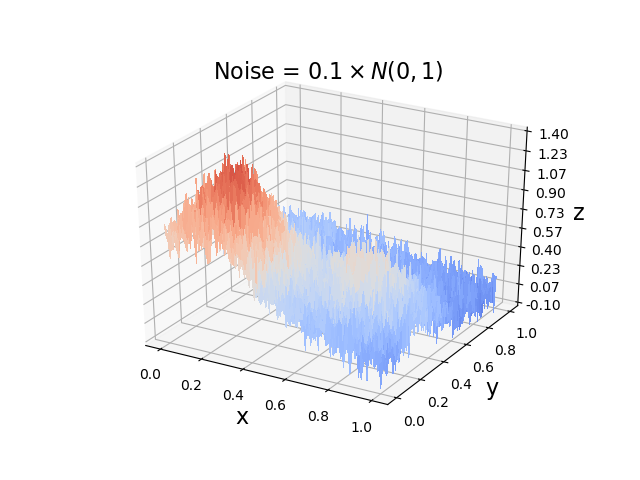
\includegraphics[width=0.50\textwidth]{original_noise.png}
    \caption{The Franke function with added noise. The noise are random numbers drawn from a Gaussian distribution $N(0,1)$.}
    \label{franke: nosie}
\end{figure}

\subsubsection{Regression: OLS}
We studied OLS by varying the maximum degree of the polynomials used in the model. Degrees 0 to 5 were used, and their results evaluated using \ref{MSE} and \ref{R2}. First without resampling, and then with both train-test split and $k$-fold cross validation.

Both the resampling methods were done using methods from \texttt{ScikitLearn}, specifically \texttt{train\_test\_split()} and \texttt{KFold}. The reaos for this was that they proved difficult to implement from scratch.

The confidence interval was computed using the following formula from (citaiton)
\begin{equation}
	\beta_j \pm z^{1 - \alpha}v_j^{1/2}\sigma
\end{equation}
where $z^{1 - \alpha}$ is the $1 - \alpha$ percentile of the normal/Gaussian distribution, thus we used $z^{1 - 0.025} = 1.96$. $v_j$ is the $j$th diagonal of $(X^tX)^{-1}$ and $\sigma$ is the standard deviation of the values themselves.

\subsubsection{Regression: Ridge}
We did the same procedure for Ridge, but we only used $k$-fold cross validation as resampling. Also, since Ridge contains a hyperparameter $\lambda$, we performed a grid search, and we produce a heat map with $MSE$ as a function of polynomial degree (model complexity) and $\lambda$. We let the degree vary between 0 and 5, and $\lambda \in [10^{-4}, 10]$.

\subsubsection{Regression: LASSO}
We used \texttt{ScikitLearn} for this method, specifically the \texttt{Lasso} method. Once again we did a grid search for the hypermarameter, and let $\lambda \in [10^{-2}, 10^{-1}]$. Note that the hyperparameter is called $\alpha$ in the program.

\section{Results}
Figures \ref{ols: 0} to \ref{ols: 5} shows the results of OLS without the use of any resampling techniques. Table \ref{table} shows the $\beta$ vector with the associated confidence intervals for each entry. Figure \ref{ols: mse} shows the MSE as a function of model complexity, that is the degree of the polynomial.

Figure \ref{ridge: mse_map} shows the result of the Ridge method. The heat map shows $MSE$ as a function of $\lambda$ and polynomial degree.

Figure \ref{lasso: mse_map} shows the result of the Ridge method. The heat map shows $MSE$ as a function of $\lambda$ and polynomial degree.

Table \ref{table_mse} displays the lowest $MSE$ score for the three methods with $k$-fold cross validation, along with the best value for their respective hyperparameters.



\begin{table}[h]  % h = "here"  , h! = here!
\caption{The $\vect{\beta}$ that minimizes the cost function, using OLS. No resampling.}\label{table}
\begin{tabular}{|c|c|c|} % note that & separates columns while \\ separates the rows
\hline                    % creates a horizontal line (try removing it)
$\beta$ entry & value & 95\% confidence  \\
\hline
0 & 0.435072 & $\pm$ 0.00378377\\                                                                                        1 &  7.48767 & $\pm$  0.0423837\\                                                                                          2 &  3.52444 & $\pm$ 0.0423837\\                                                                                          3 & -33.1635 & $\pm$  0.204656\\                                                                                          4 &  -13.862 & $\pm$  0.159838\\                                                                                5 & -7.96259 & $\pm$  0.204656\\                                                                                          6 &  46.9101 & $\pm$ 0.459742\\                              7 &  41.6446 & $\pm$  0.340723\\                                                                                          8 &  19.0085 & $\pm$  0.340723\\                                                                                          9 & -9.04219 & $\pm$  0.459742\\                                                                                         10 & -23.2623 & $\pm$   0.480122\\                                                                                         11 & -50.6661 & $\pm$  0.366568\\                                                                                         12 & -5.51051 & $\pm$  0.341091\\                                                                                         13 & -28.5962 & $\pm$  0.366568\\                                                                                         14 &  29.9243 & $\pm$  0.480122\\                                                                                         15 &  1.64575 & $\pm$  0.188273\\                                                                                         16 &  18.2115 & $\pm$  0.163674\\                                                                                         17 &  9.41273 & $\pm$  0.159634\\                                                                                         18 & -5.75018 & $\pm$  0.159634\\                                                                                         19 &   16.364 & $\pm$  0.163674\\                                                                                         20 & -16.7033 & $\pm$  0.188273\\  
\hline
\end{tabular}
\end{table}


\begin{table}[h]  % h = "here"  , h! = here!
\caption{MSE scores for OLS, Ridge and LASSO methods.}\label{table_mse}
\begin{tabular}{|c|c|c|} % note that & separates columns while \\ separates the rows
\hline                    % creates a horizontal line (try removing it)
Method & MSE & Hypermarameter  \\
\hline
OLS &    0.0120786 & -\\                                                                                        Ridge &  0.0120865 & $\lambda \approx$ 0.0001\\                                               
LASSO &  0.2556345 & $\lambda \approx$ 0.0774264\\ 
 \hline
\end{tabular}
\end{table}

\begin{figure}[h]
    \centering
    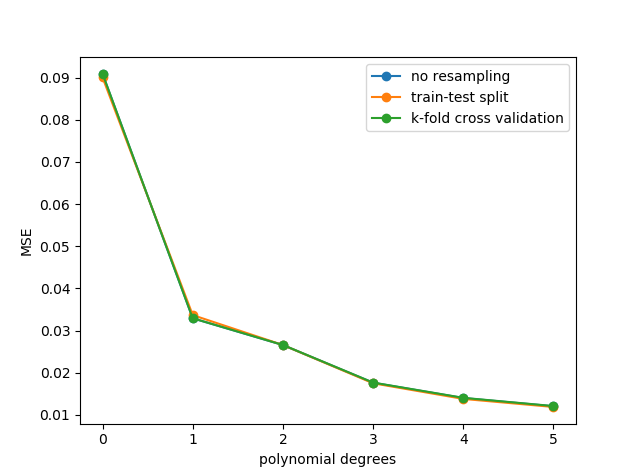
\includegraphics[width=0.50\textwidth]{OLS_mse.png}
    \caption{MSE of the OLS method, without resampling, with train-test split and with k-fold cross validation.}
    \label{ols: mse}
\end{figure}


\begin{figure}[h]
    \centering
    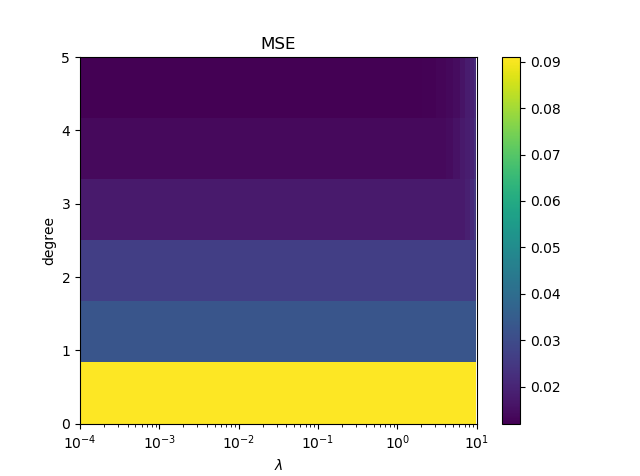
\includegraphics[width=0.50\textwidth]{RIDGE_mse.png}
    \caption{MSE of the Ridge method, with k-fold cross validation.}
    \label{ridge: mse_map}
\end{figure}

\begin{figure}[h]
    \centering
    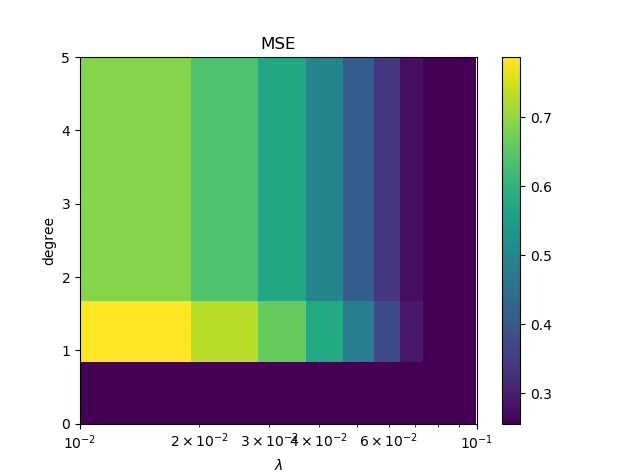
\includegraphics[width=0.50\textwidth]{LASSO_mse.png}
    \caption{MSE of the LASSO method, with k-fold cross validation.}
    \label{lasso: mse_map}
\end{figure}



\section{Conclusion}
It is clear from table \ref{table_mse} that OLS is the method that best fits the kind of data we look at in this project. It has the lowest MSE score, although not by much. Ridge also performs nearly as well, but it should be pointed out that the hyperparameter is very small, in fact the smallest tested value, suggesting that the penalty term makes the model less accurate. 



\section*{References}
\begin{itemize}
\item[-] https://www.uio.no/studier/emner/matnat/astro/\
AST2000/h19/undervisningsmateriell\_h2019/\
forelesningsnotater/part1b.pdf
\end{itemize}


\begin{figure}[h]
    \centering
    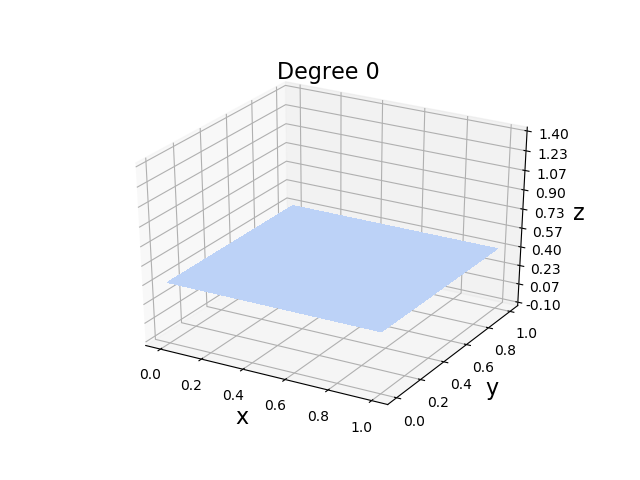
\includegraphics[width=0.50\textwidth]{OLS_deg0.png}
    \caption{Franke function approximated by polonimials of degree 0.}
    \label{ols: 0}
\end{figure}

\begin{figure}[h]
    \centering
    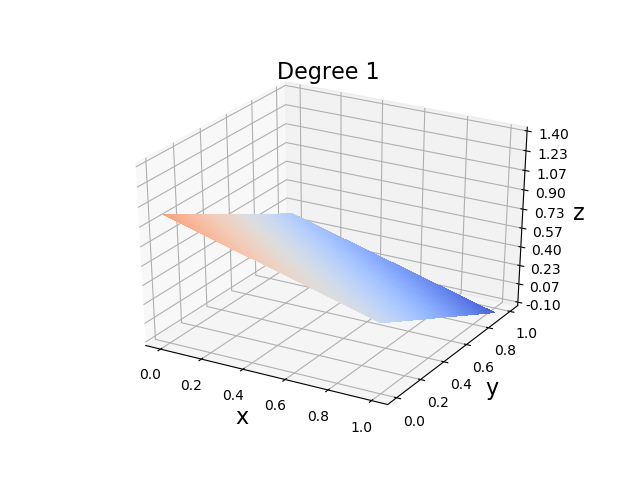
\includegraphics[width=0.50\textwidth]{OLS_deg1.png}
    \caption{Franke function approximated by polonimials of degree 1.}
    \label{ols: 1}
\end{figure}

\begin{figure}[h]
    \centering
    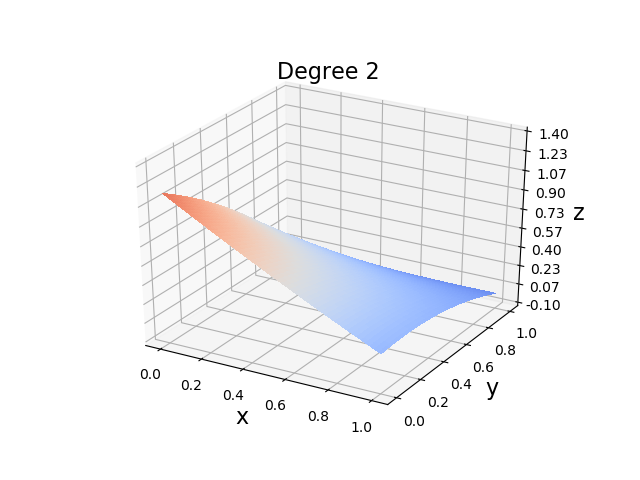
\includegraphics[width=0.50\textwidth]{OLS_deg2.png}
    \caption{Franke function approximated by polonimials of degree 2.}
    \label{ols: 2}
\end{figure}

\begin{figure}[h]
    \centering
    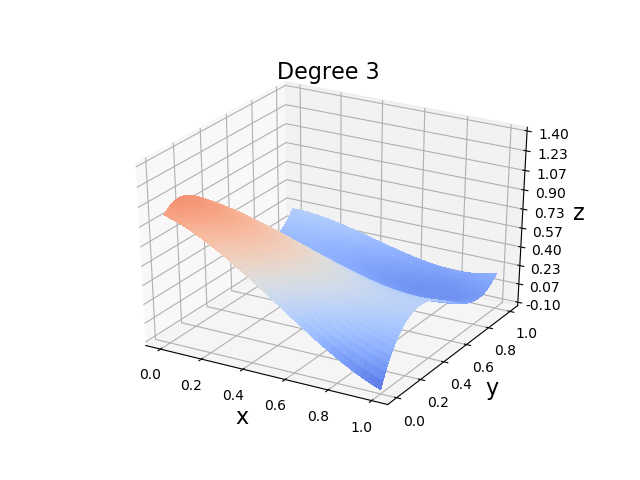
\includegraphics[width=0.50\textwidth]{OLS_deg3.png}
    \caption{Franke function approximated by polonimials of degree 3.}
    \label{ols: 3}
\end{figure}

\begin{figure}[h]
    \centering
    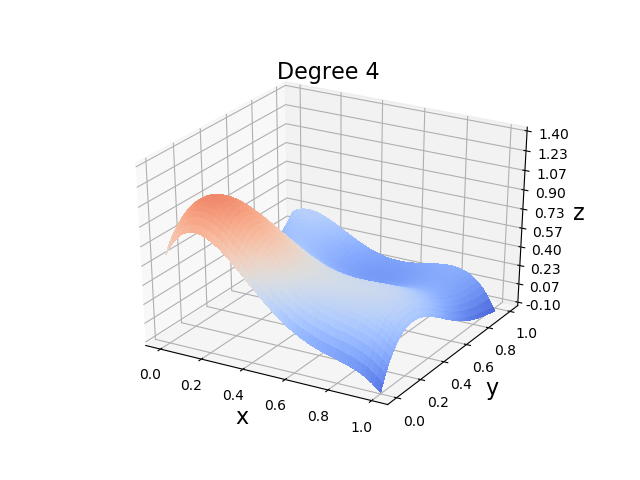
\includegraphics[width=0.50\textwidth]{OLS_deg4.png}
    \caption{Franke function approximated by polonimials of degree 4.}
    \label{ols: 4}
\end{figure}

\begin{figure}[h]
    \centering
    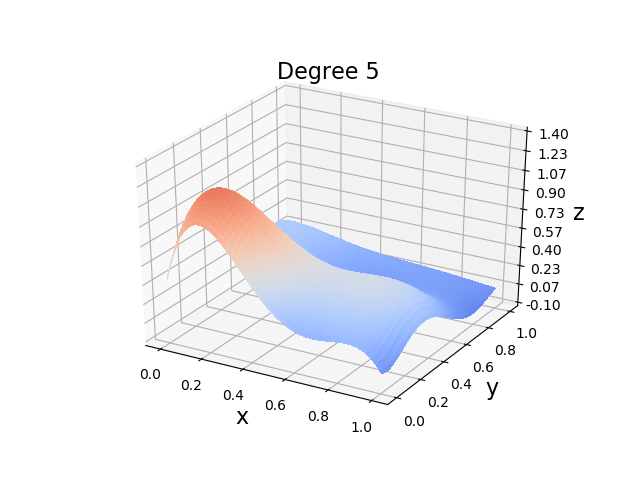
\includegraphics[width=0.50\textwidth]{OLS_deg5.png}
    \caption{Franke function approximated by polonimials of degree 5.}
    \label{ols: 5}
\end{figure}


\end{document}
